\documentclass{article}
\usepackage{amsfonts} 
\usepackage{hyperref}
\usepackage{graphicx}

\begin{document}


\section{Model}
\par The probabilistic model is simple. The first we just generate the cloud of $n$ points uniformly distributed in $[0, 1]^d$. After this we calculate the Alpha complex with these points, and then find its depth poset.

\section{Scores}
\subsection{Poset Scores}
\begin{itemize}
\item \textbf{number\_of\_nodes }: Returns the number of nodes in the poset.
\item \textbf{number\_of\_relations }: Returns the number of relations in the transitive reduction.
\item \textbf{number\_of\_components }: Returns the number of connetcted components in the poset
\item \textbf{cycles\_dimension }: Returns the dimension of space of cycles in reduction.
\item \textbf{number\_of\_minimal\_nodes }: Returns the number of minimal nodes.
\item \textbf{number\_of\_maximal\_nodes }: Returns the number of maximal nodes.
\item \textbf{height }: Returns the poset height - the length of the longest chain.
\item \textbf{width }: Returns the poset width - the length of the longest antichain (subset, s.t. all elements are pairwise incomparable).
    The algorithm is based on Dilworth's theorem and it's proof via Kőnig's theorem:
    \href{https://en.wikipedia.org/wiki/Dilworth%27s_theorem}{link}
\item \textbf{minimum\_maximal\_chain }: Returns the minimum size of maximal chains in the poset.
\item \textbf{avarage\_maximal\_chain }: Returns the avarage size of maximal chains in the poset.
\end{itemize}

\subsection{Node Scores}
\begin{itemize}
\item \textbf{ancestors\_number}: Returns the number of nodes higher than given
\item \textbf{ancestors\_height}: Returns the size of maximum chain of subposet of nodes higher or equal than given
\item \textbf{ancestors\_width}: Returns the size of maximum chain of subposet of nodes higher or equal than given
\item \textbf{ancestors\_cycles\_dimension}: Returns the the dimension of space of cycles in reduction of subposet of nodes higher or equal than given
\item \textbf{successors\_number}: Returns the number of nodes higher than given
\item \textbf{successors\_height}: Returns the size of maximum chain of subposet of nodes lower or equal than given
\item \textbf{successors\_width}: Returns the size of maximum chain of subposet of nodes lower or equal than given
\item \textbf{successors\_cycles\_dimension}: Returns the the dimension of space of cycles in reduction of subposet of nodes lower or equal than given
\end{itemize}

\section{Experiments and Results}
\par There are 1119 experiments done. In the Figure \ref{fig:cases_distribution} we can see how cases are distributed by size and dimension.
\begin{figure}[ht]
  \centering
  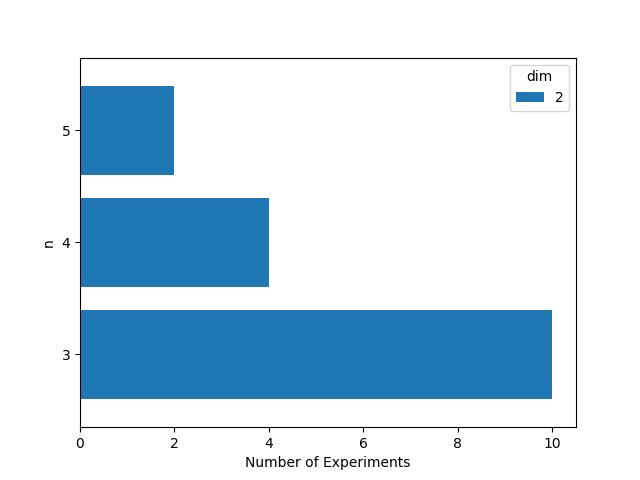
\includegraphics[width=\textwidth]{pics/scores - cases.png}
  \caption{Size/dimension distribution of experiments}
  \label{fig:cases_distribution}
\end{figure}

\subsection{Depth Poset Features}
\par In the Figure \ref{fig:scores_poset_mean} we can see the avarage poset scores values for each number of points $n$ in the depth poset.
\begin{figure}[ht]
  \vspace{-96pt}
  \centering
  \hspace*{-0.18999999999999995\textwidth}
  \resizebox{1.38\textwidth}{!}{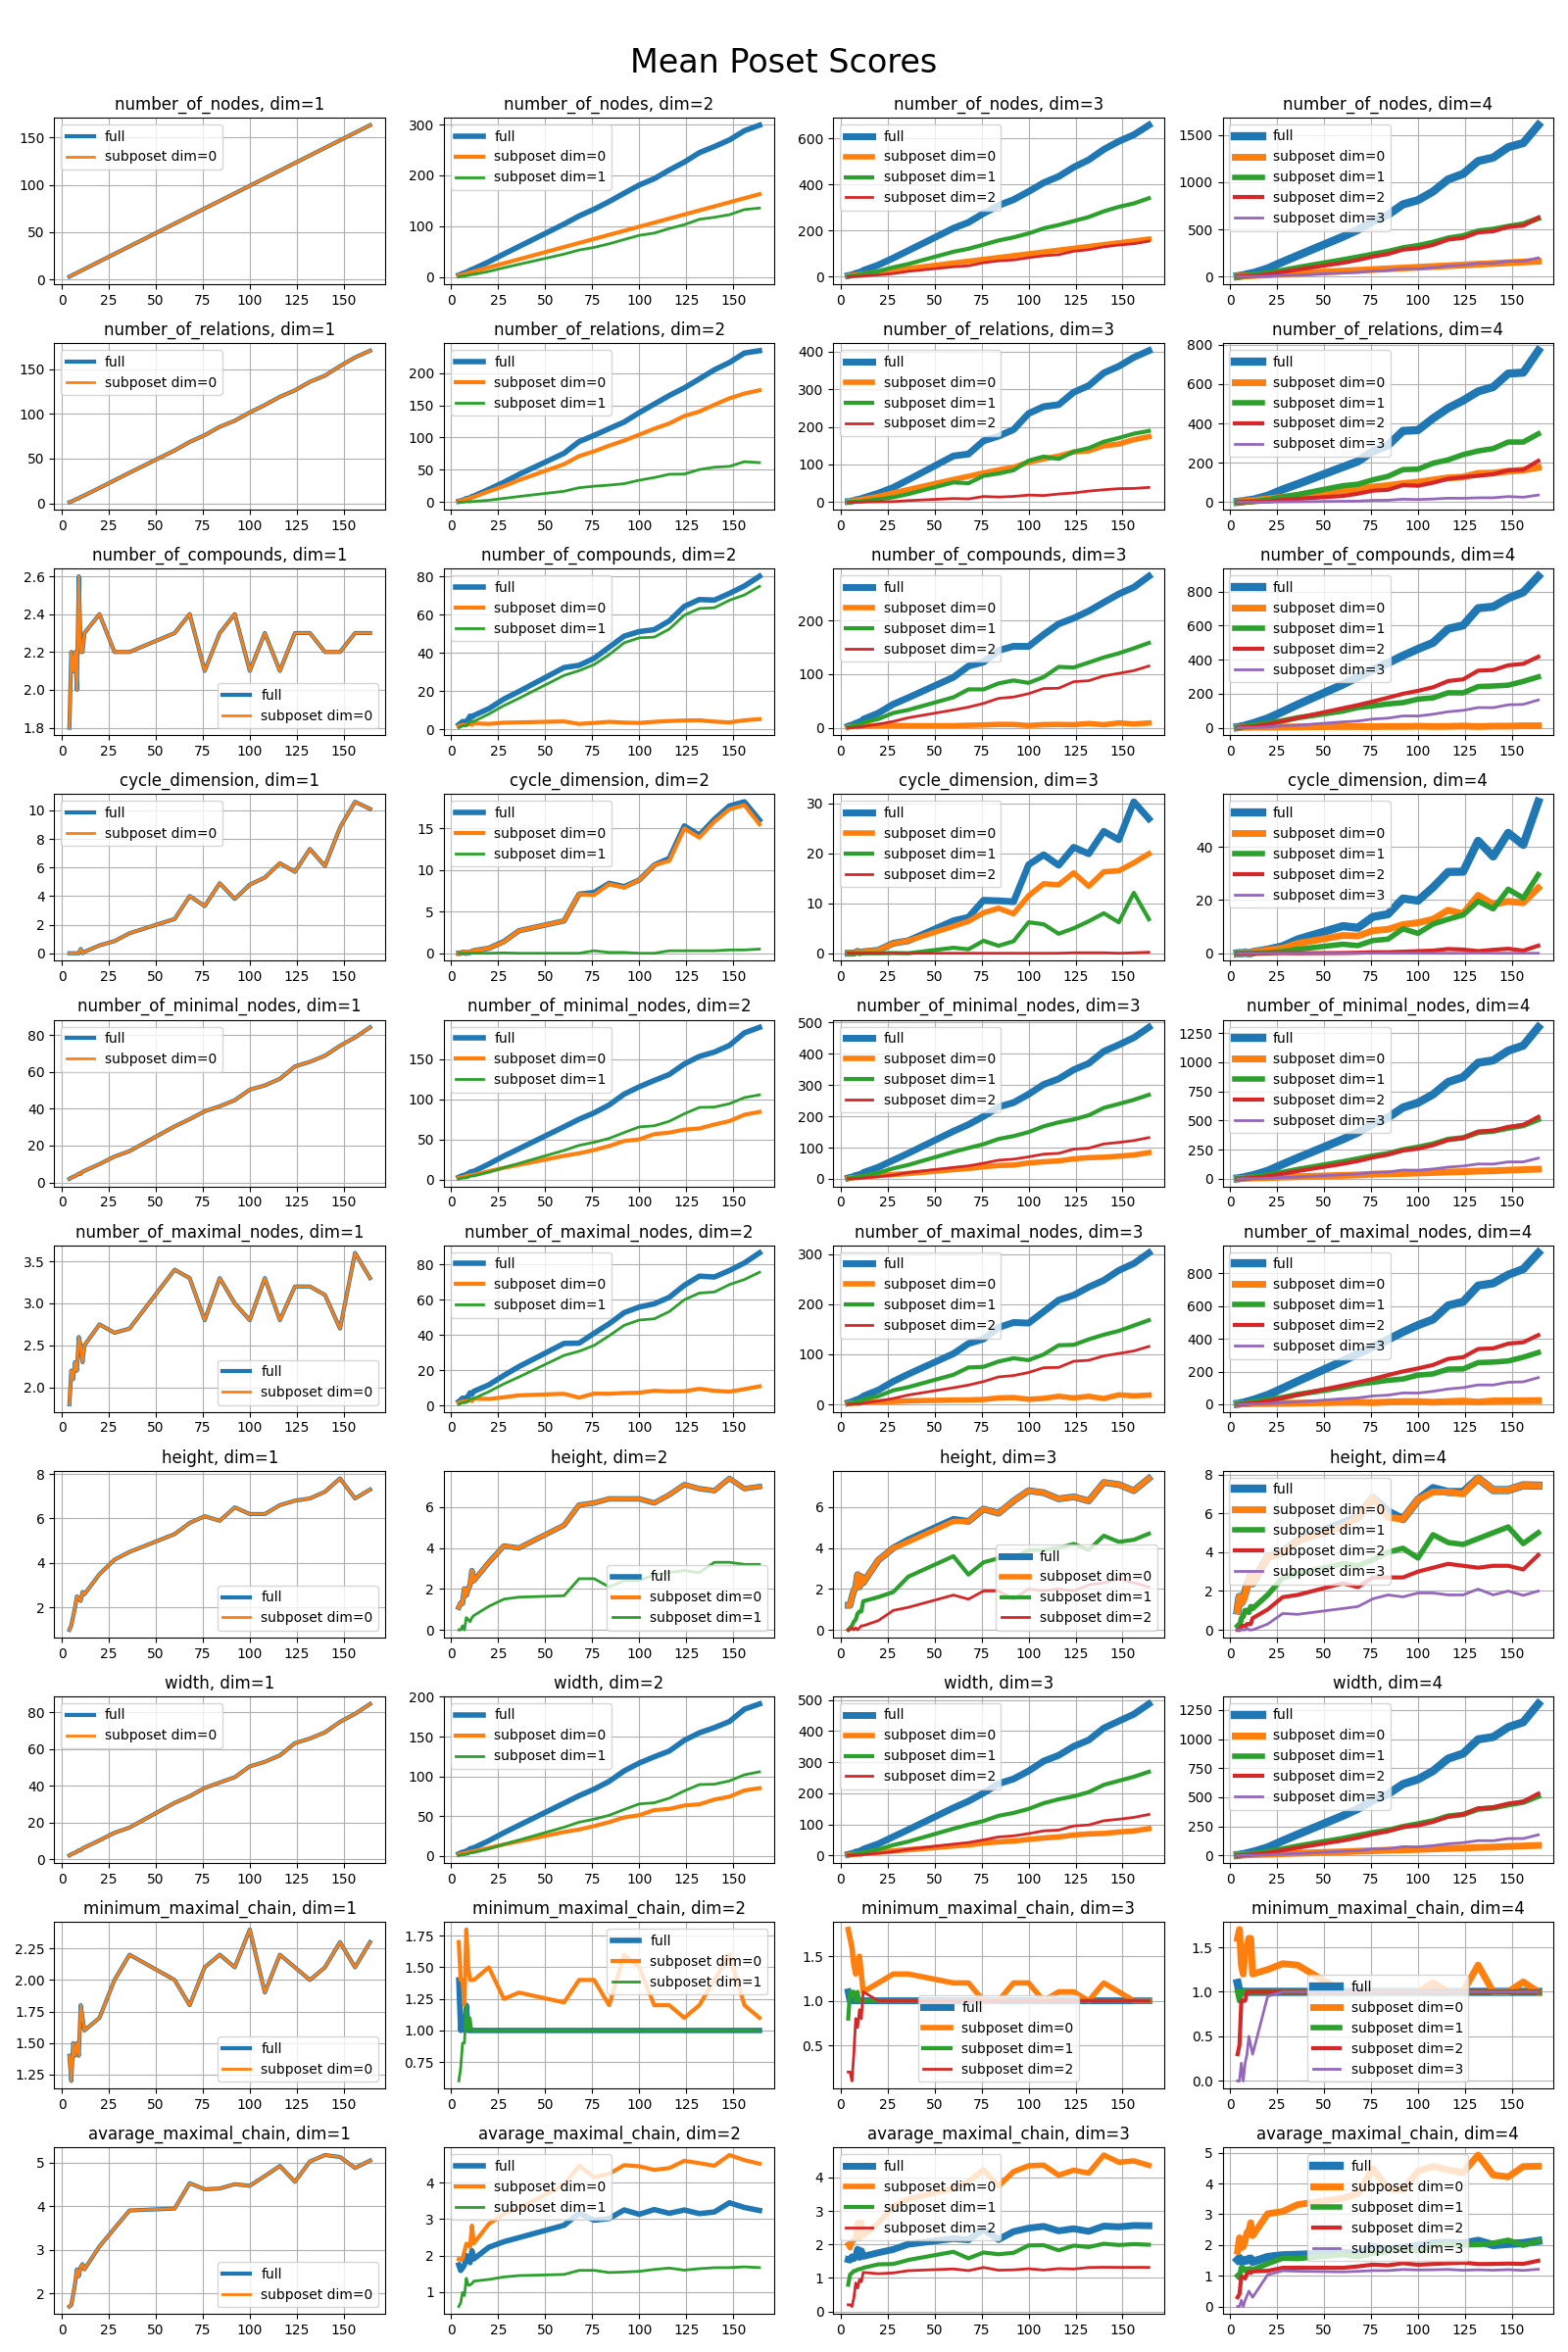
\includegraphics[width=\textwidth]{pics/scores - mean poset scores.png}}
  \caption{Depth Poset: Mean poset scores}
  \label{fig:scores_poset_mean}
\end{figure}

\par In the Figure \ref{fig:scores_node_mean} we can see the avarage mean node scores values in poset for each number of points $n$ in the depth poset.
\begin{figure}[ht]
  \vspace{-96pt}
  \centering
  \hspace*{-0.18999999999999995\textwidth}
  \resizebox{1.38\textwidth}{!}{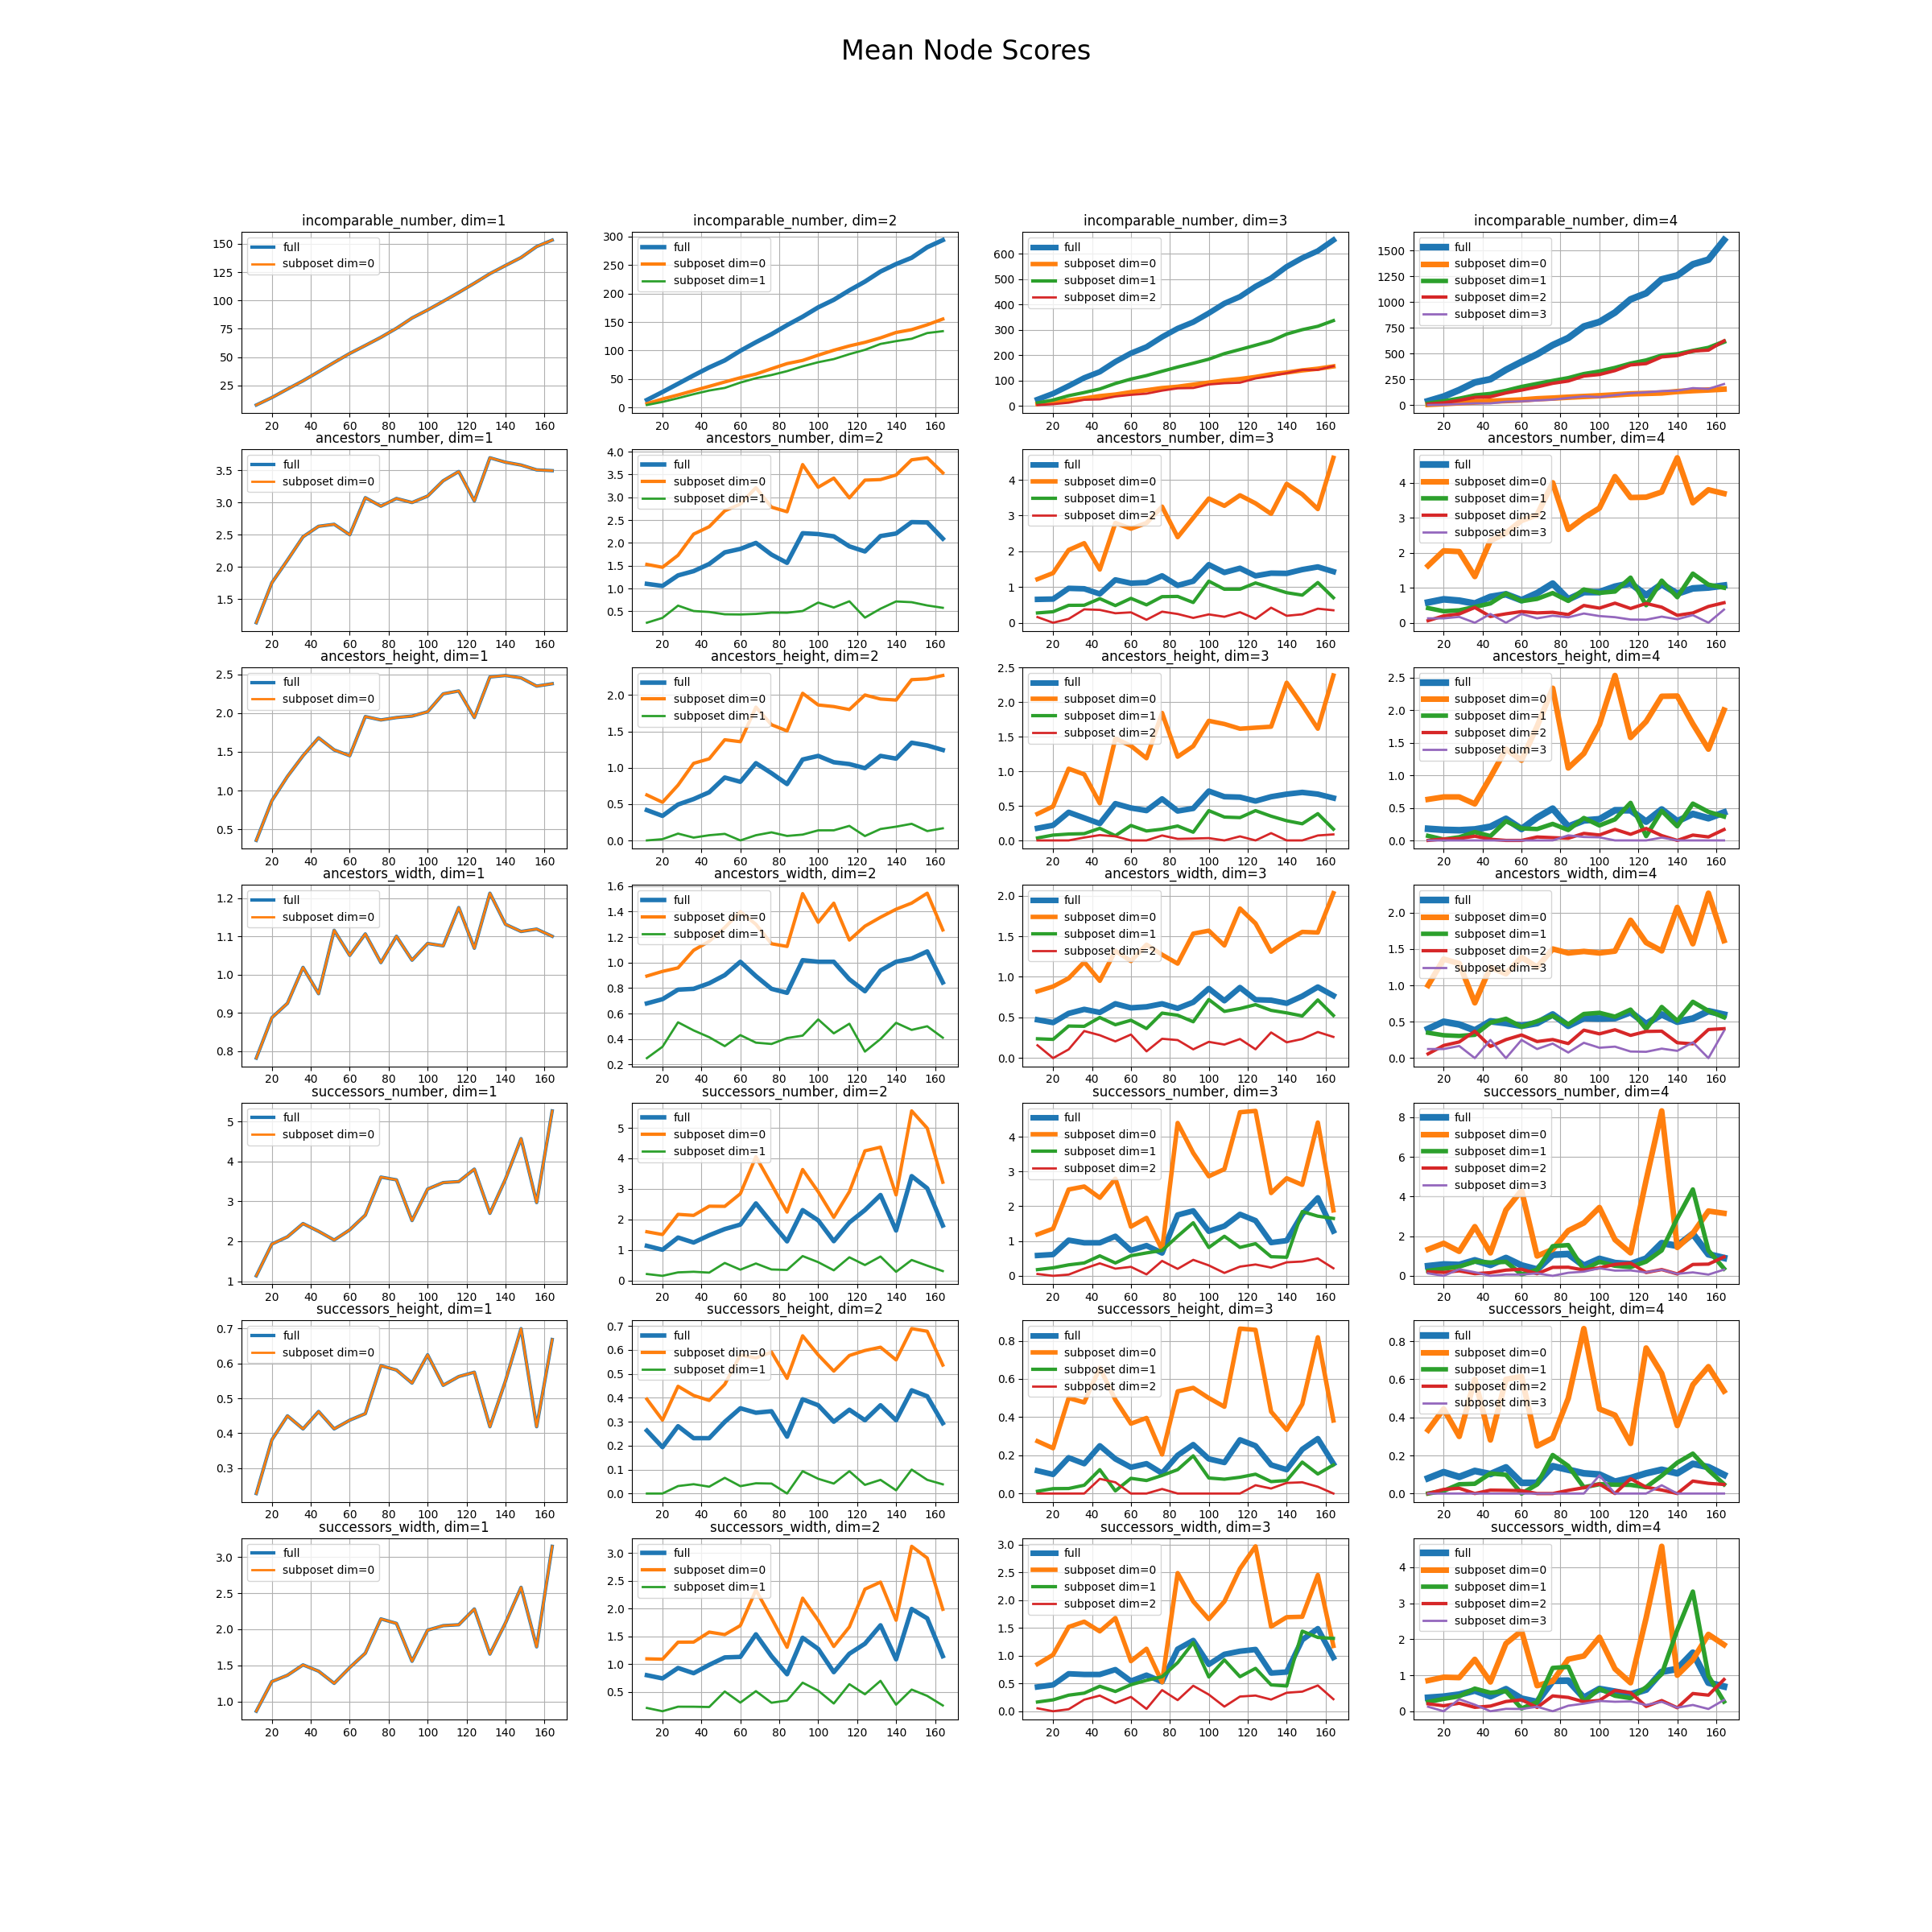
\includegraphics[width=\textwidth]{pics/scores - mean node scores.png}}
  \caption{Depth Poset: Mean node scores}
  \label{fig:scores_node_mean}
\end{figure}

\par In the Figure \ref{fig:scores_node_max} we can see the avarage maximum node scores values in poset for each number of points $n$ in the depth poset.
\begin{figure}[ht]
  \vspace{-96pt}
  \centering
  \hspace*{-0.18999999999999995\textwidth}
  \resizebox{1.38\textwidth}{!}{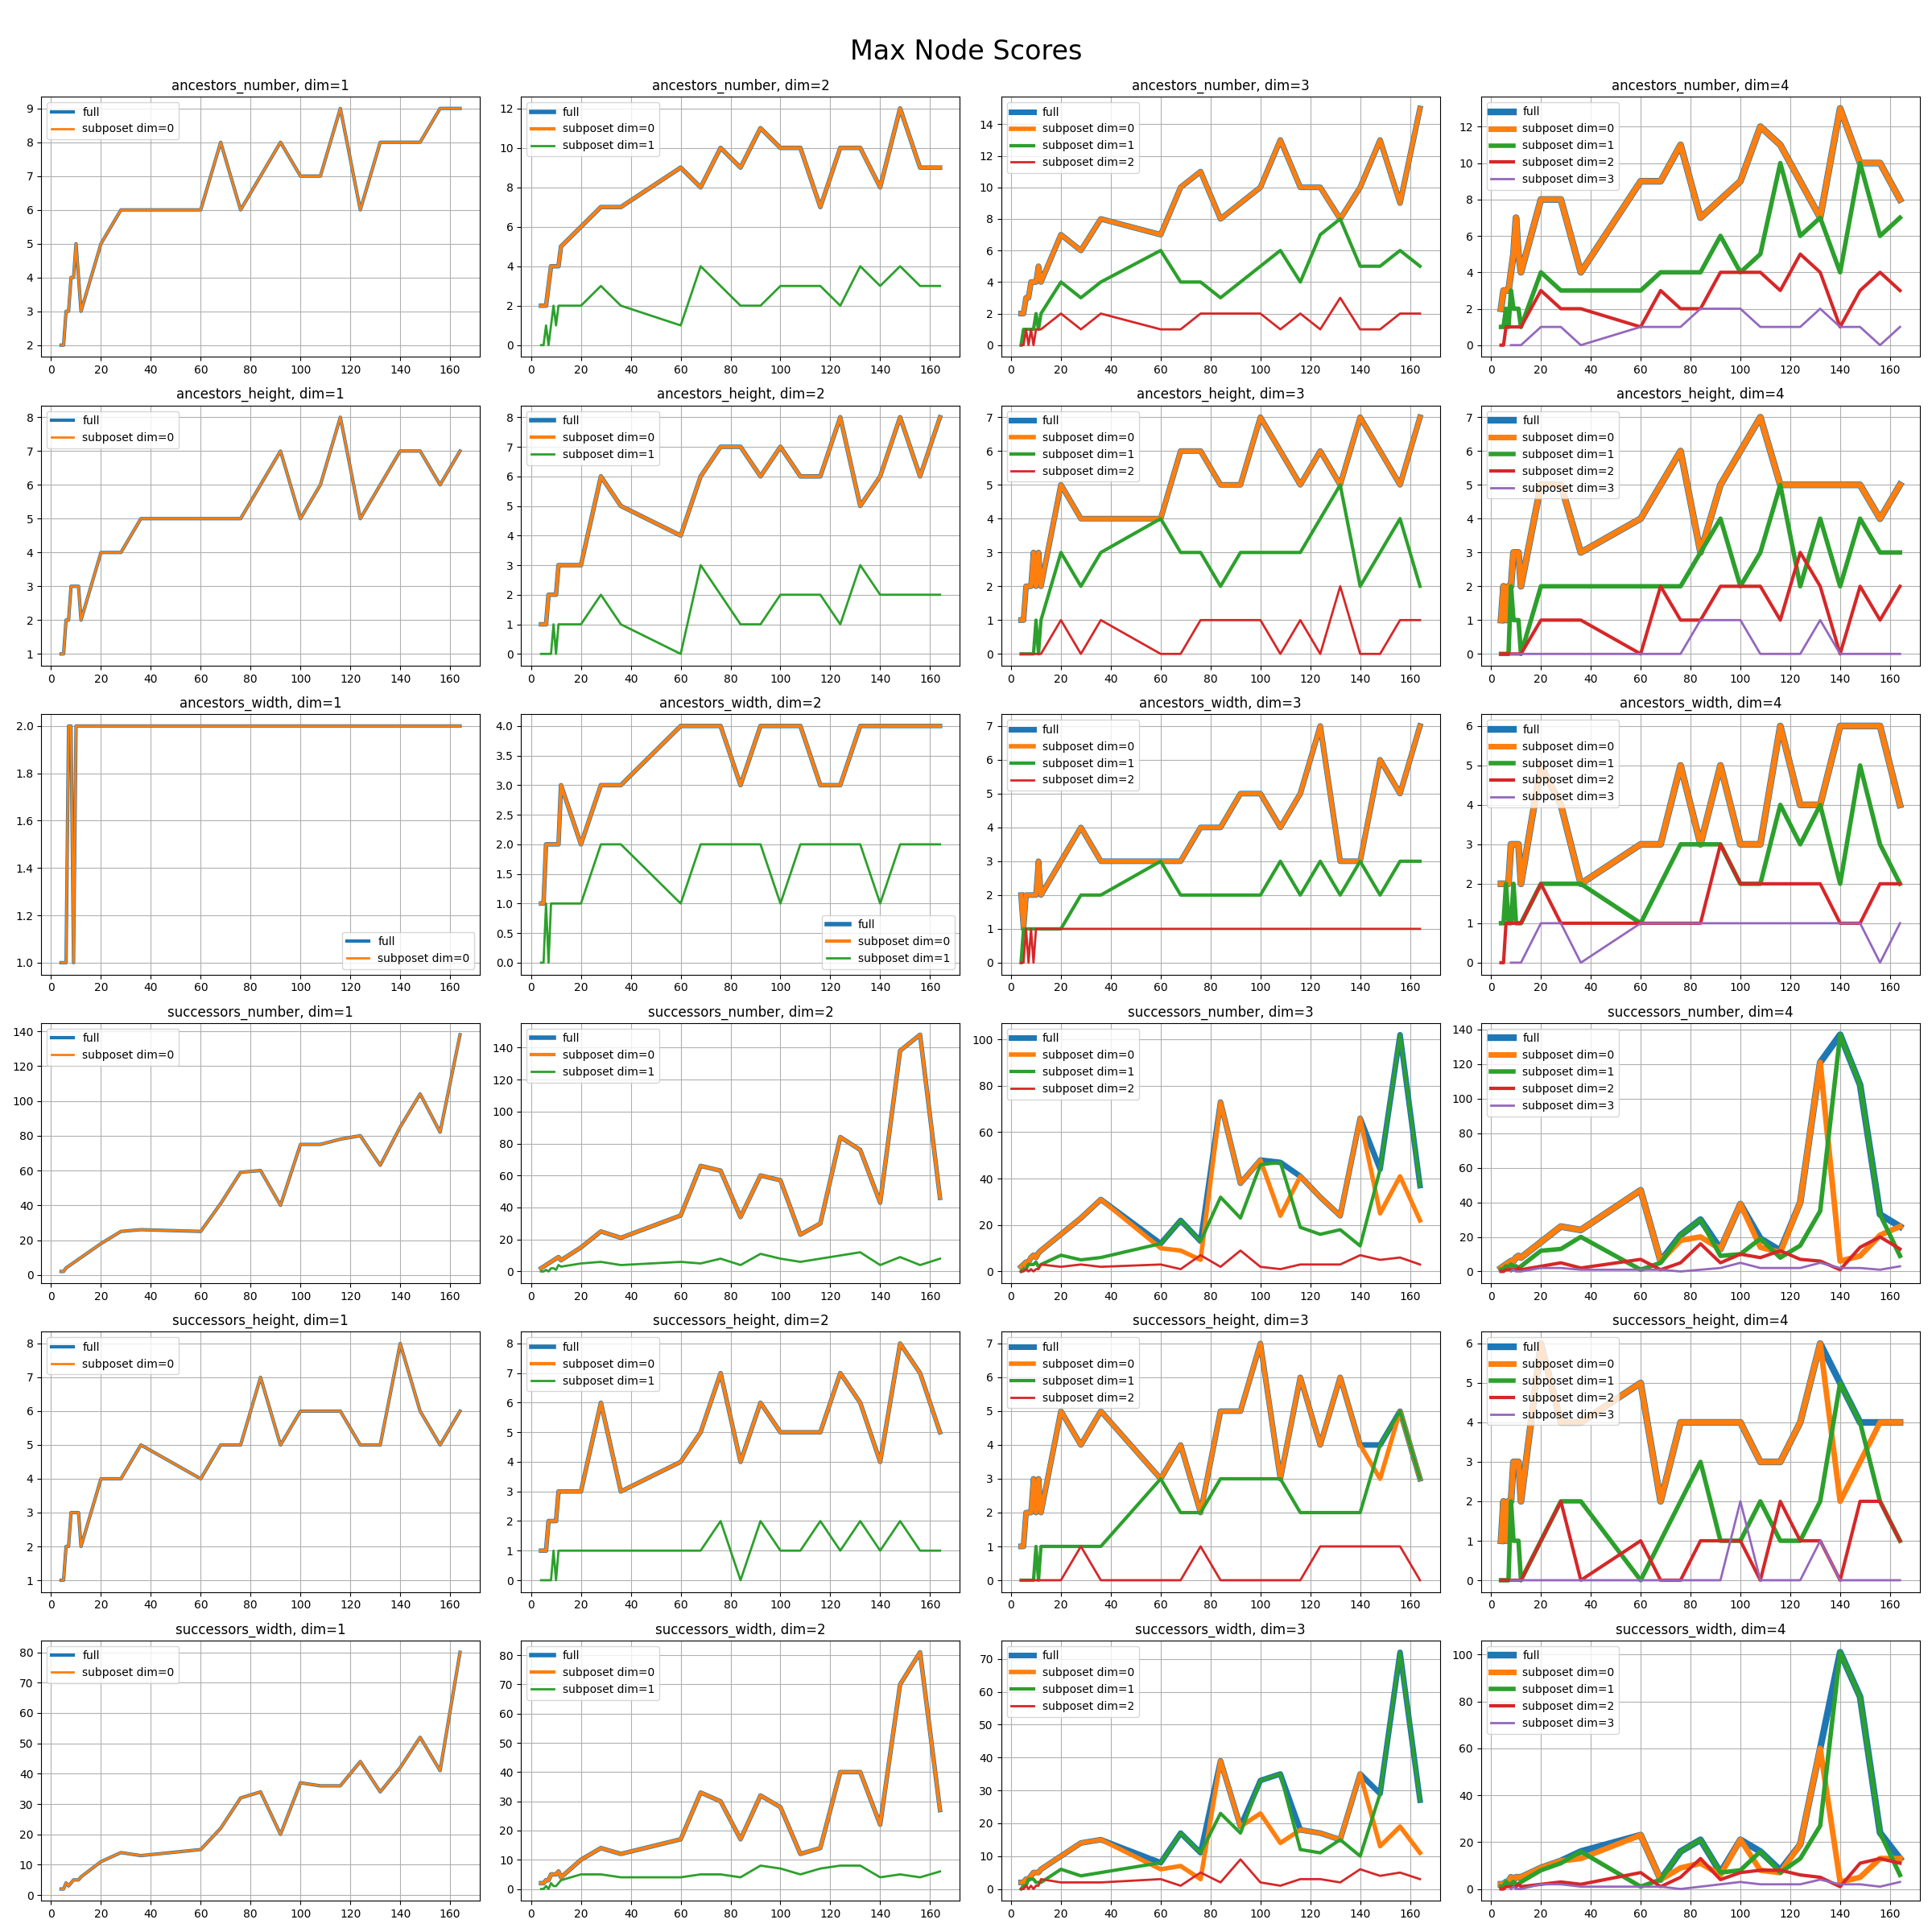
\includegraphics[width=\textwidth]{pics/scores - max node scores.png}}
  \caption{Depth Poset: Max node scores}
  \label{fig:scores_node_max}
\end{figure}

\subsection{Column Reduction Poset Features}
\par In the Figure \ref{fig:scores_poset_mean_crp} we can see the avarage poset scores values for each number of points $n$ in the column reduction poset.
\begin{figure}[ht]
  \vspace{-96pt}
  \centering
  \hspace*{-0.18999999999999995\textwidth}
  \resizebox{1.38\textwidth}{!}{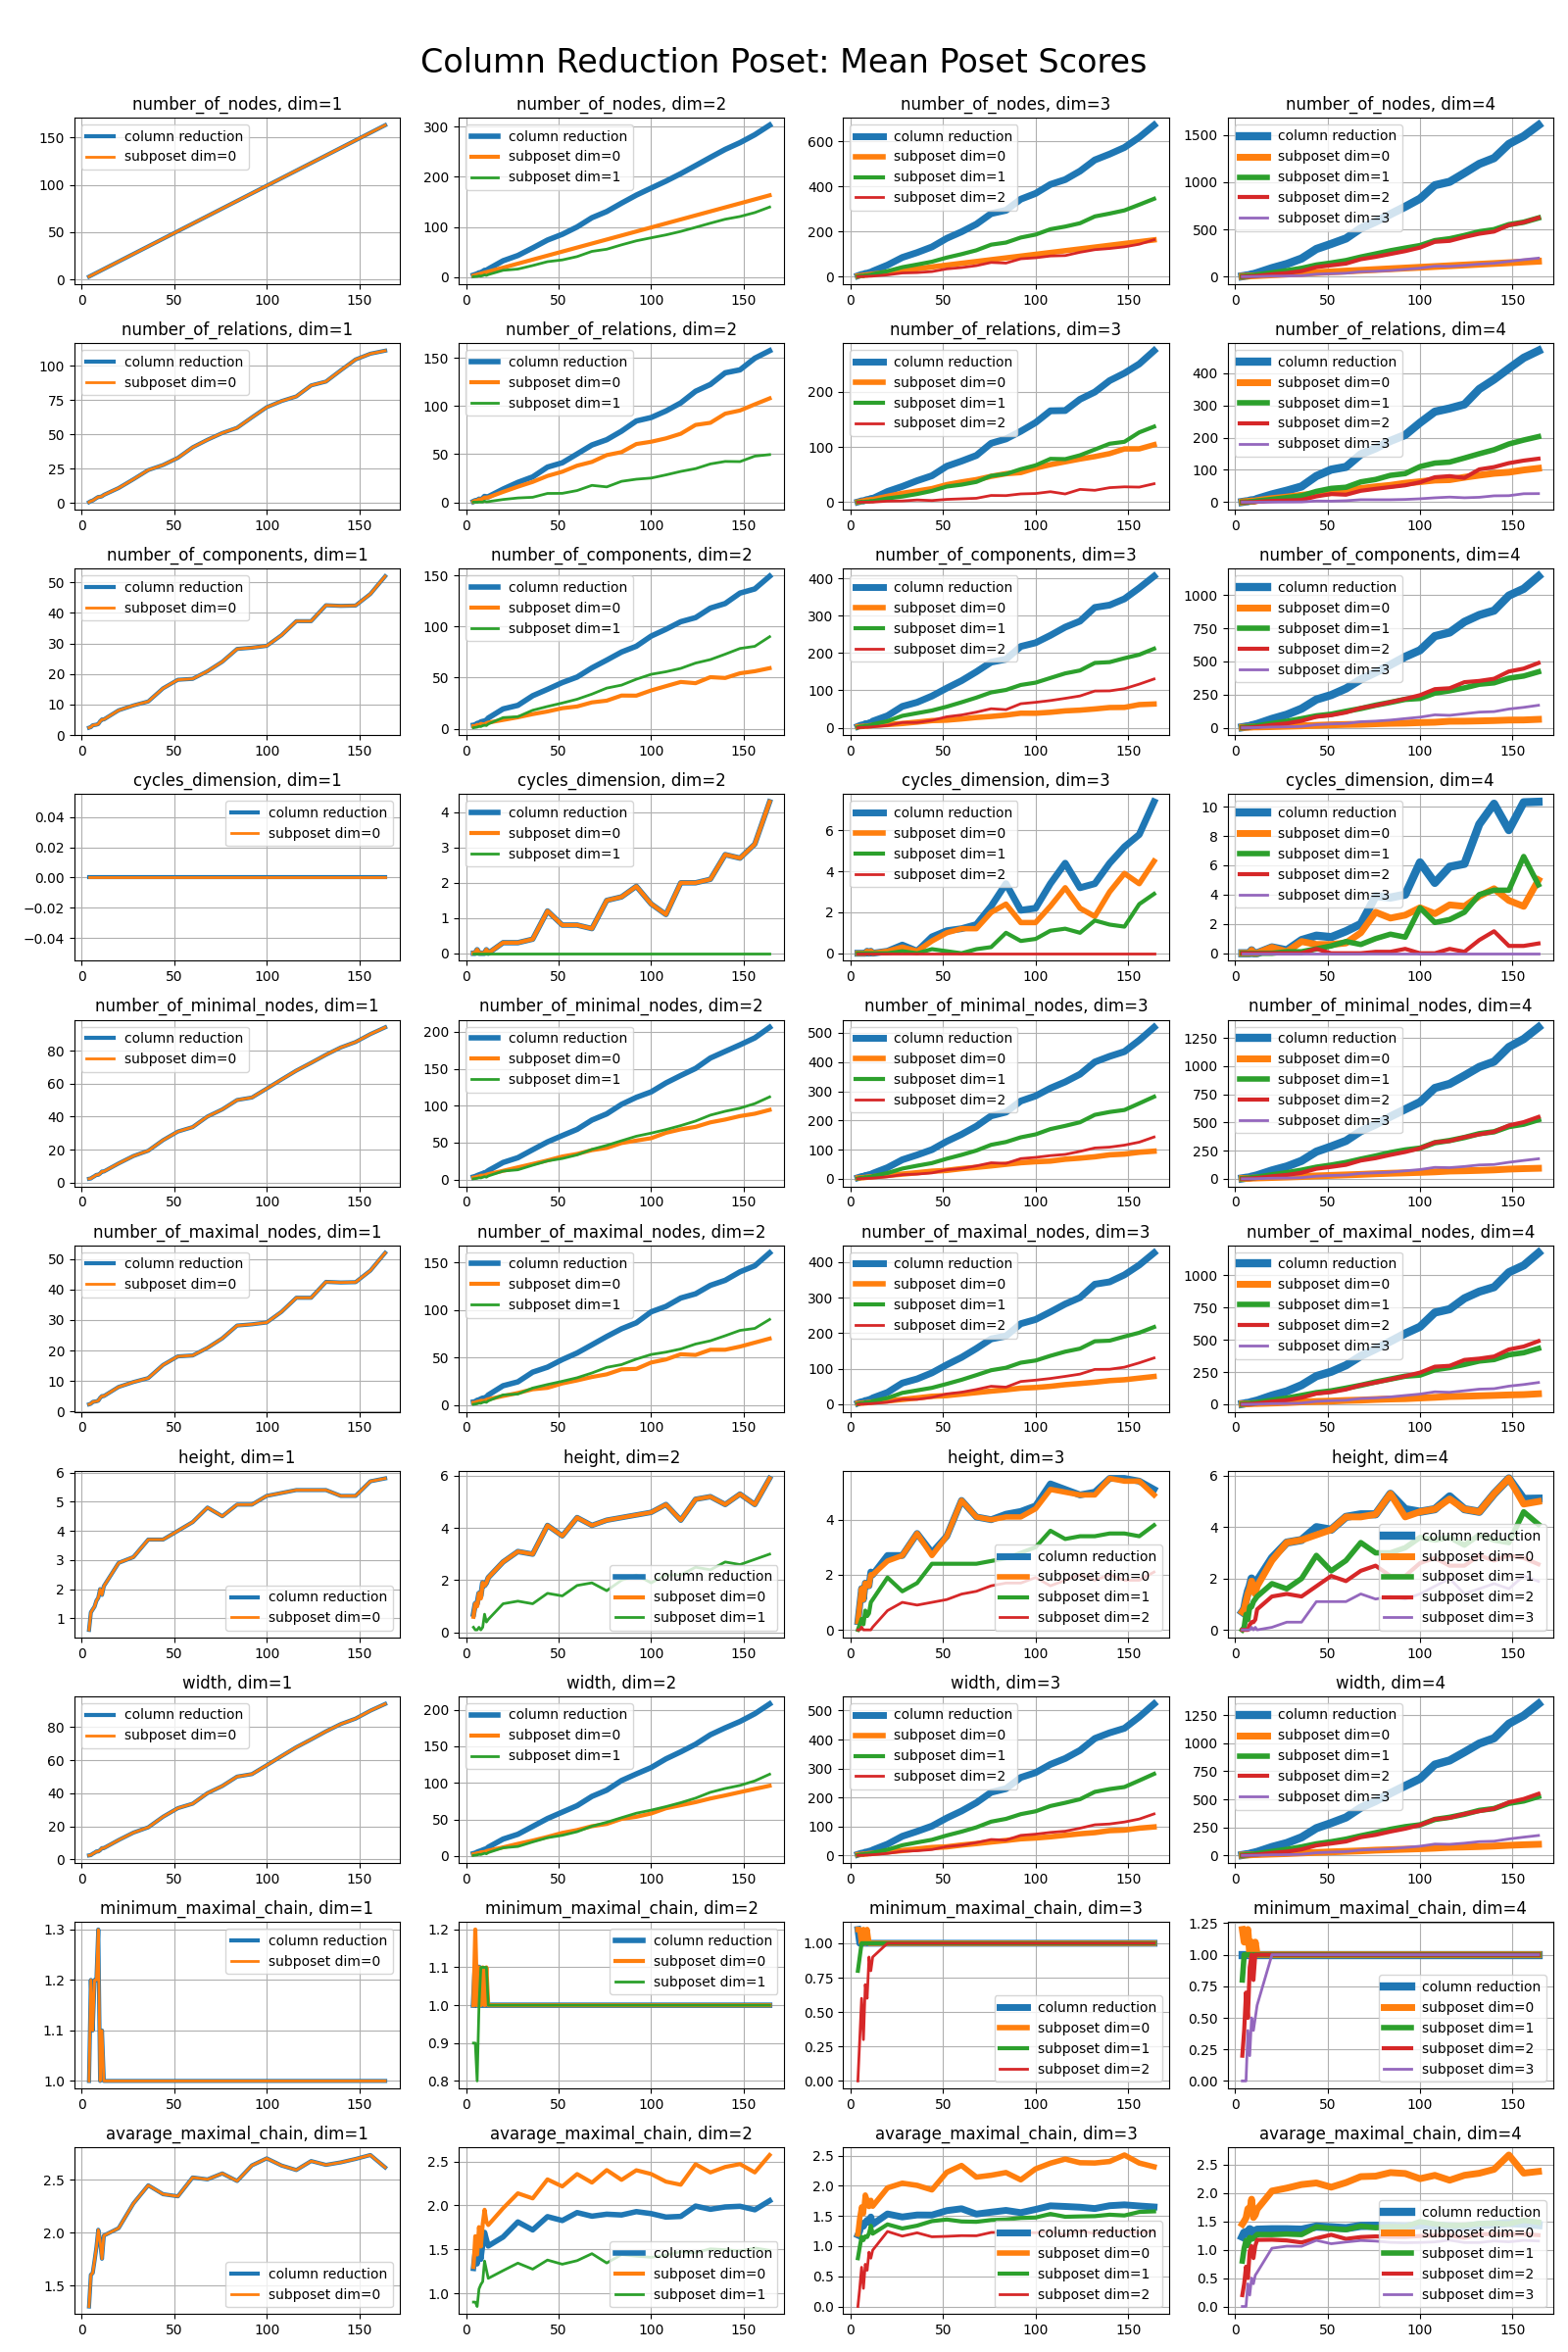
\includegraphics[width=\textwidth]{pics/scores - mean poset scores - column reduction.png}}
  \caption{Column Reduction Poset: Mean poset scores}
  \label{fig:scores_poset_mean_crp}
\end{figure}

\par In the Figure \ref{fig:scores_node_mean_crp} we can see the avarage mean node scores values in poset for each number of points $n$ in the column reduction poset.
\begin{figure}[ht]
  \vspace{-96pt}
  \centering
  \hspace*{-0.18999999999999995\textwidth}
  \resizebox{1.38\textwidth}{!}{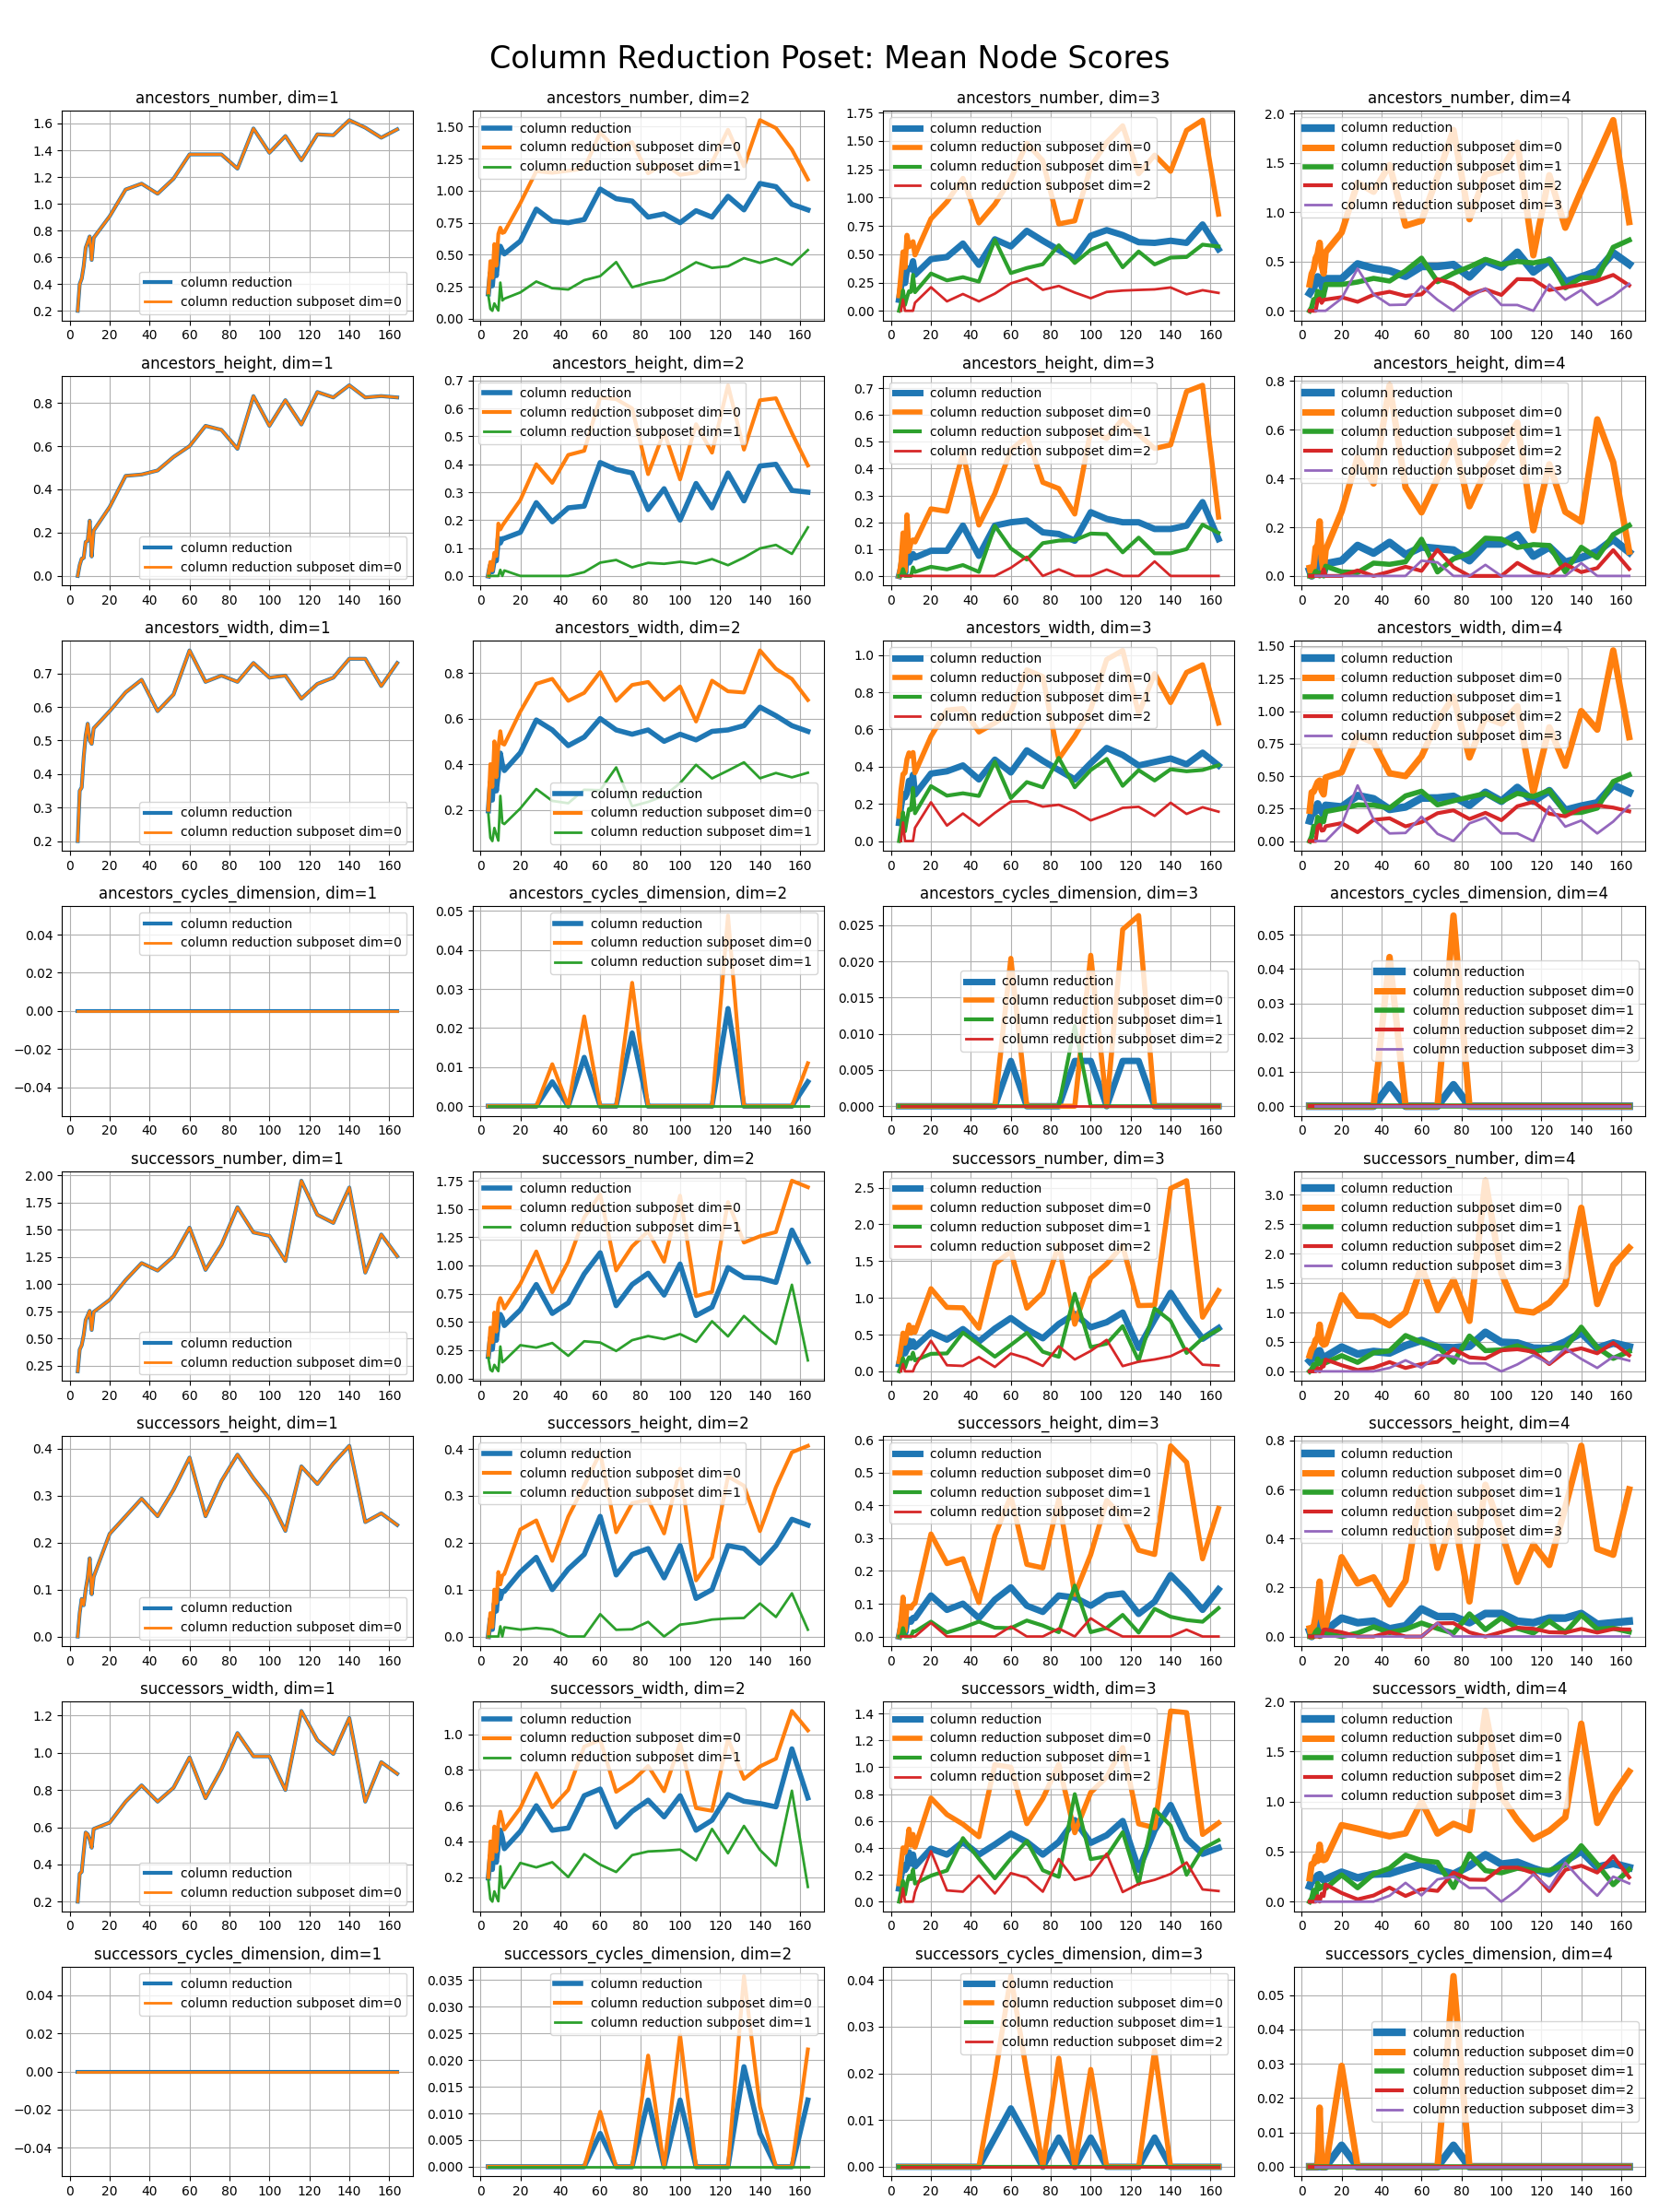
\includegraphics[width=\textwidth]{pics/scores - mean node scores - column reduction.png}}
  \caption{Column Reduction Poset: Mean node scores}
  \label{fig:scores_node_mean_crp}
\end{figure}

\par In the Figure \ref{fig:scores_node_max_crp} we can see the avarage maximum node scores values in poset for each number of points $n$ in the column reduction poset.
\begin{figure}[ht]
  \vspace{-96pt}
  \centering
  \hspace*{-0.18999999999999995\textwidth}
  \resizebox{1.38\textwidth}{!}{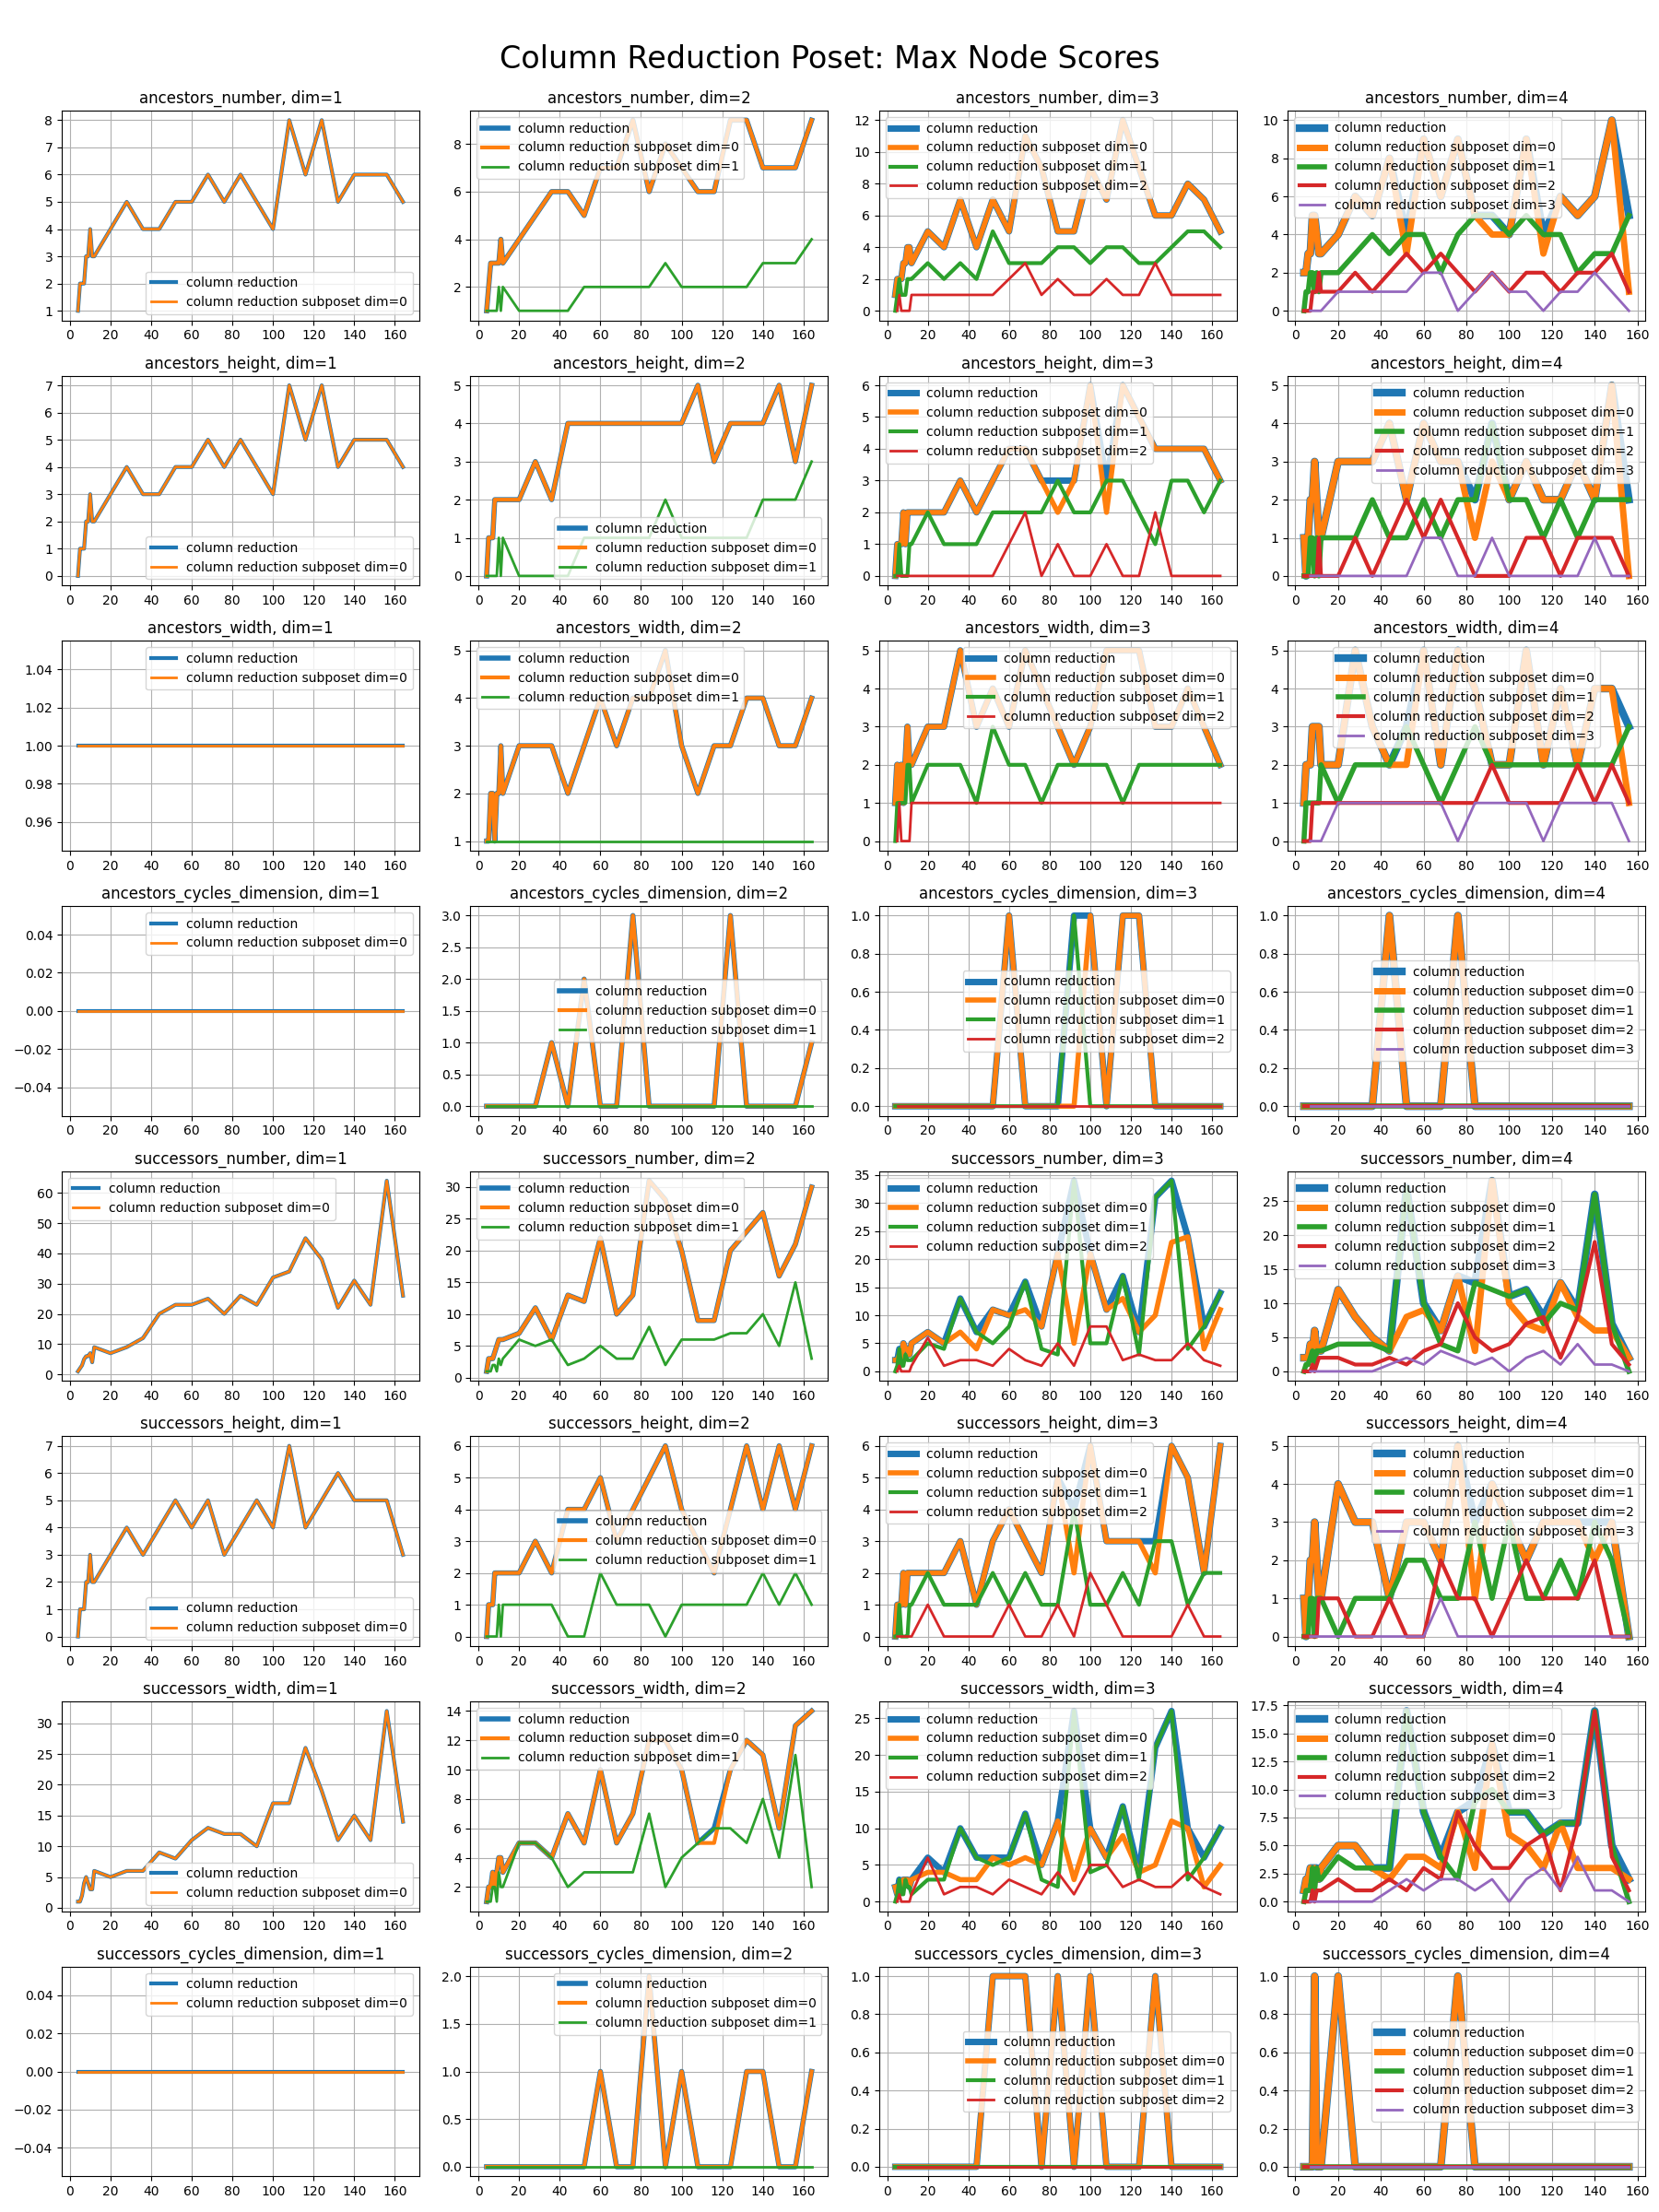
\includegraphics[width=\textwidth]{pics/scores - max node scores - column reduction.png}}
  \caption{Column Reduction Poset: Max node scores}
  \label{fig:scores_node_max_crp}
\end{figure}

\subsection{Row Reduction Poset Features}
\par In the Figure \ref{fig:scores_poset_mean_rrp} we can see the avarage poset scores values for each number of points $n$ in the row reduction poset.
\begin{figure}[ht]
  \vspace{-96pt}
  \centering
  \hspace*{-0.18999999999999995\textwidth}
  \resizebox{1.38\textwidth}{!}{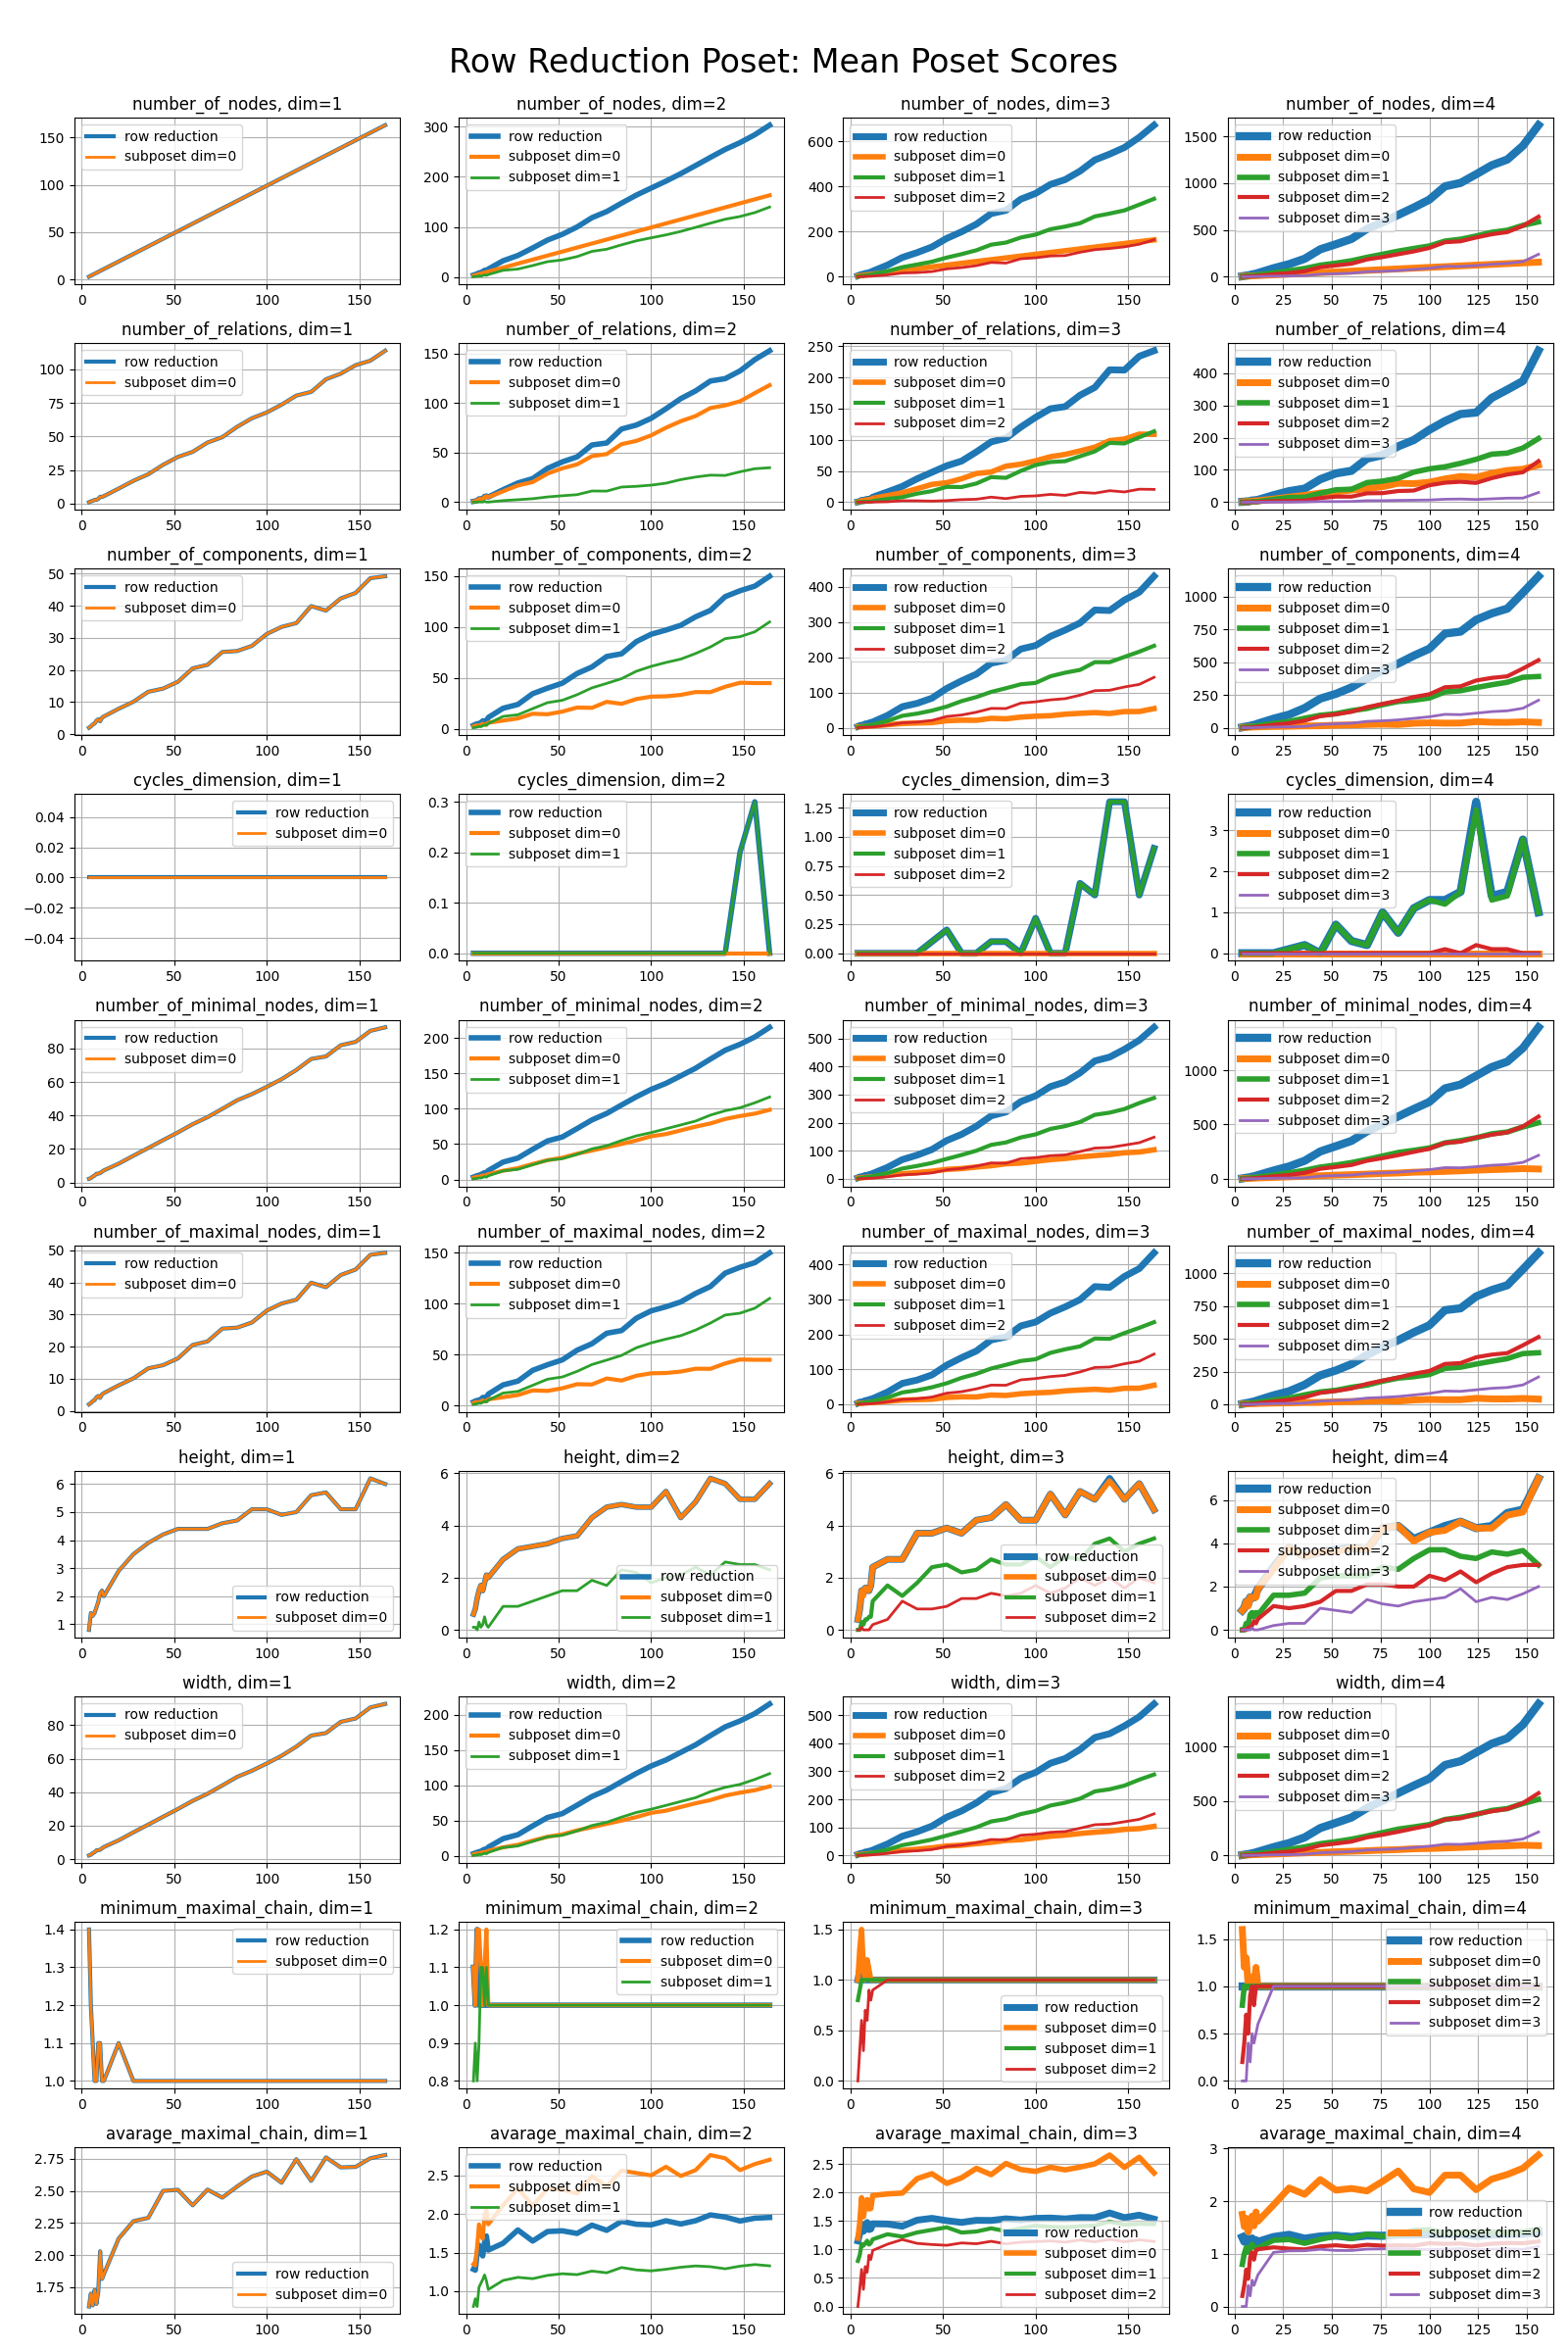
\includegraphics[width=\textwidth]{pics/scores - mean poset scores - row reduction.png}}
  \caption{Row Reduction Poset: Mean poset scores}
  \label{fig:scores_poset_mean_rrp}
\end{figure}

\par In the Figure \ref{fig:scores_node_mean_rrp} we can see the avarage mean node scores values in poset for each number of points $n$ in the row reduction poset.
\begin{figure}[ht]
  \vspace{-96pt}
  \centering
  \hspace*{-0.18999999999999995\textwidth}
  \resizebox{1.38\textwidth}{!}{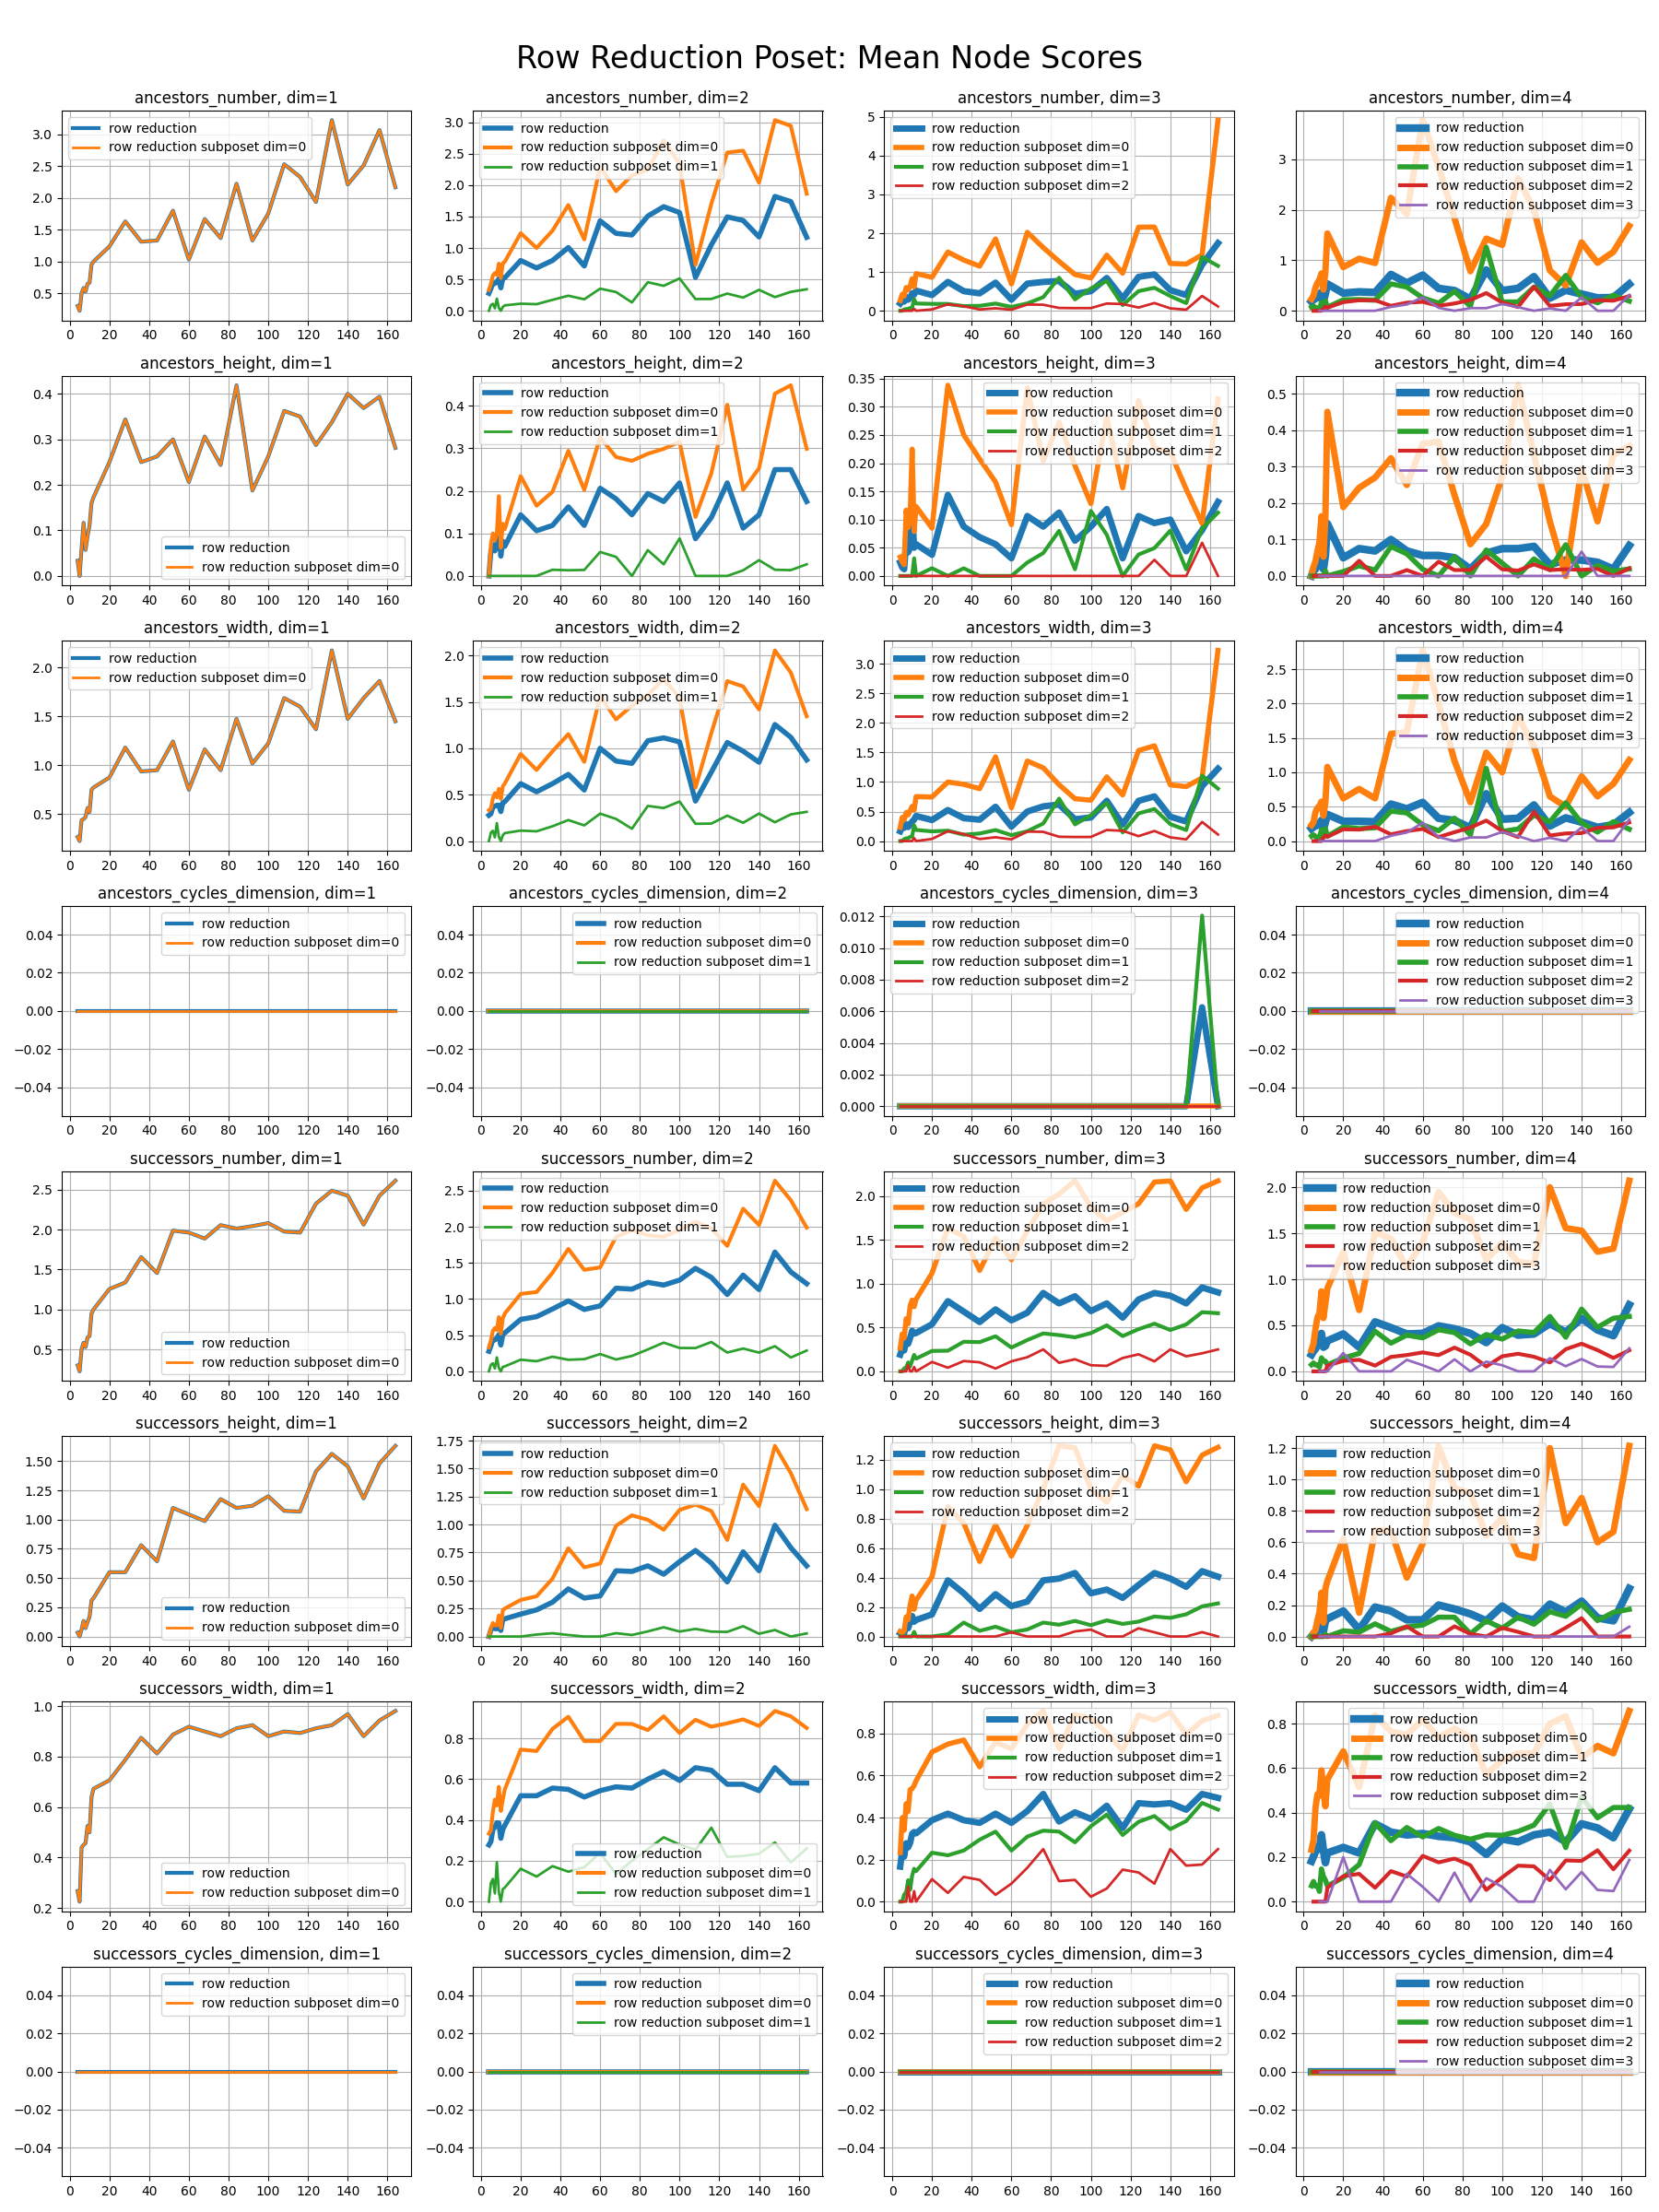
\includegraphics[width=\textwidth]{pics/scores - mean node scores - row reduction.png}}
  \caption{Row Reduction Poset: Mean node scores}
  \label{fig:scores_node_mean_rrp}
\end{figure}

\par In the Figure \ref{fig:scores_node_max_rrp} we can see the avarage maximum node scores values in poset for each number of points $n$ in the row reduction poset.
\begin{figure}[ht]
  \vspace{-96pt}
  \centering
  \hspace*{-0.18999999999999995\textwidth}
  \resizebox{1.38\textwidth}{!}{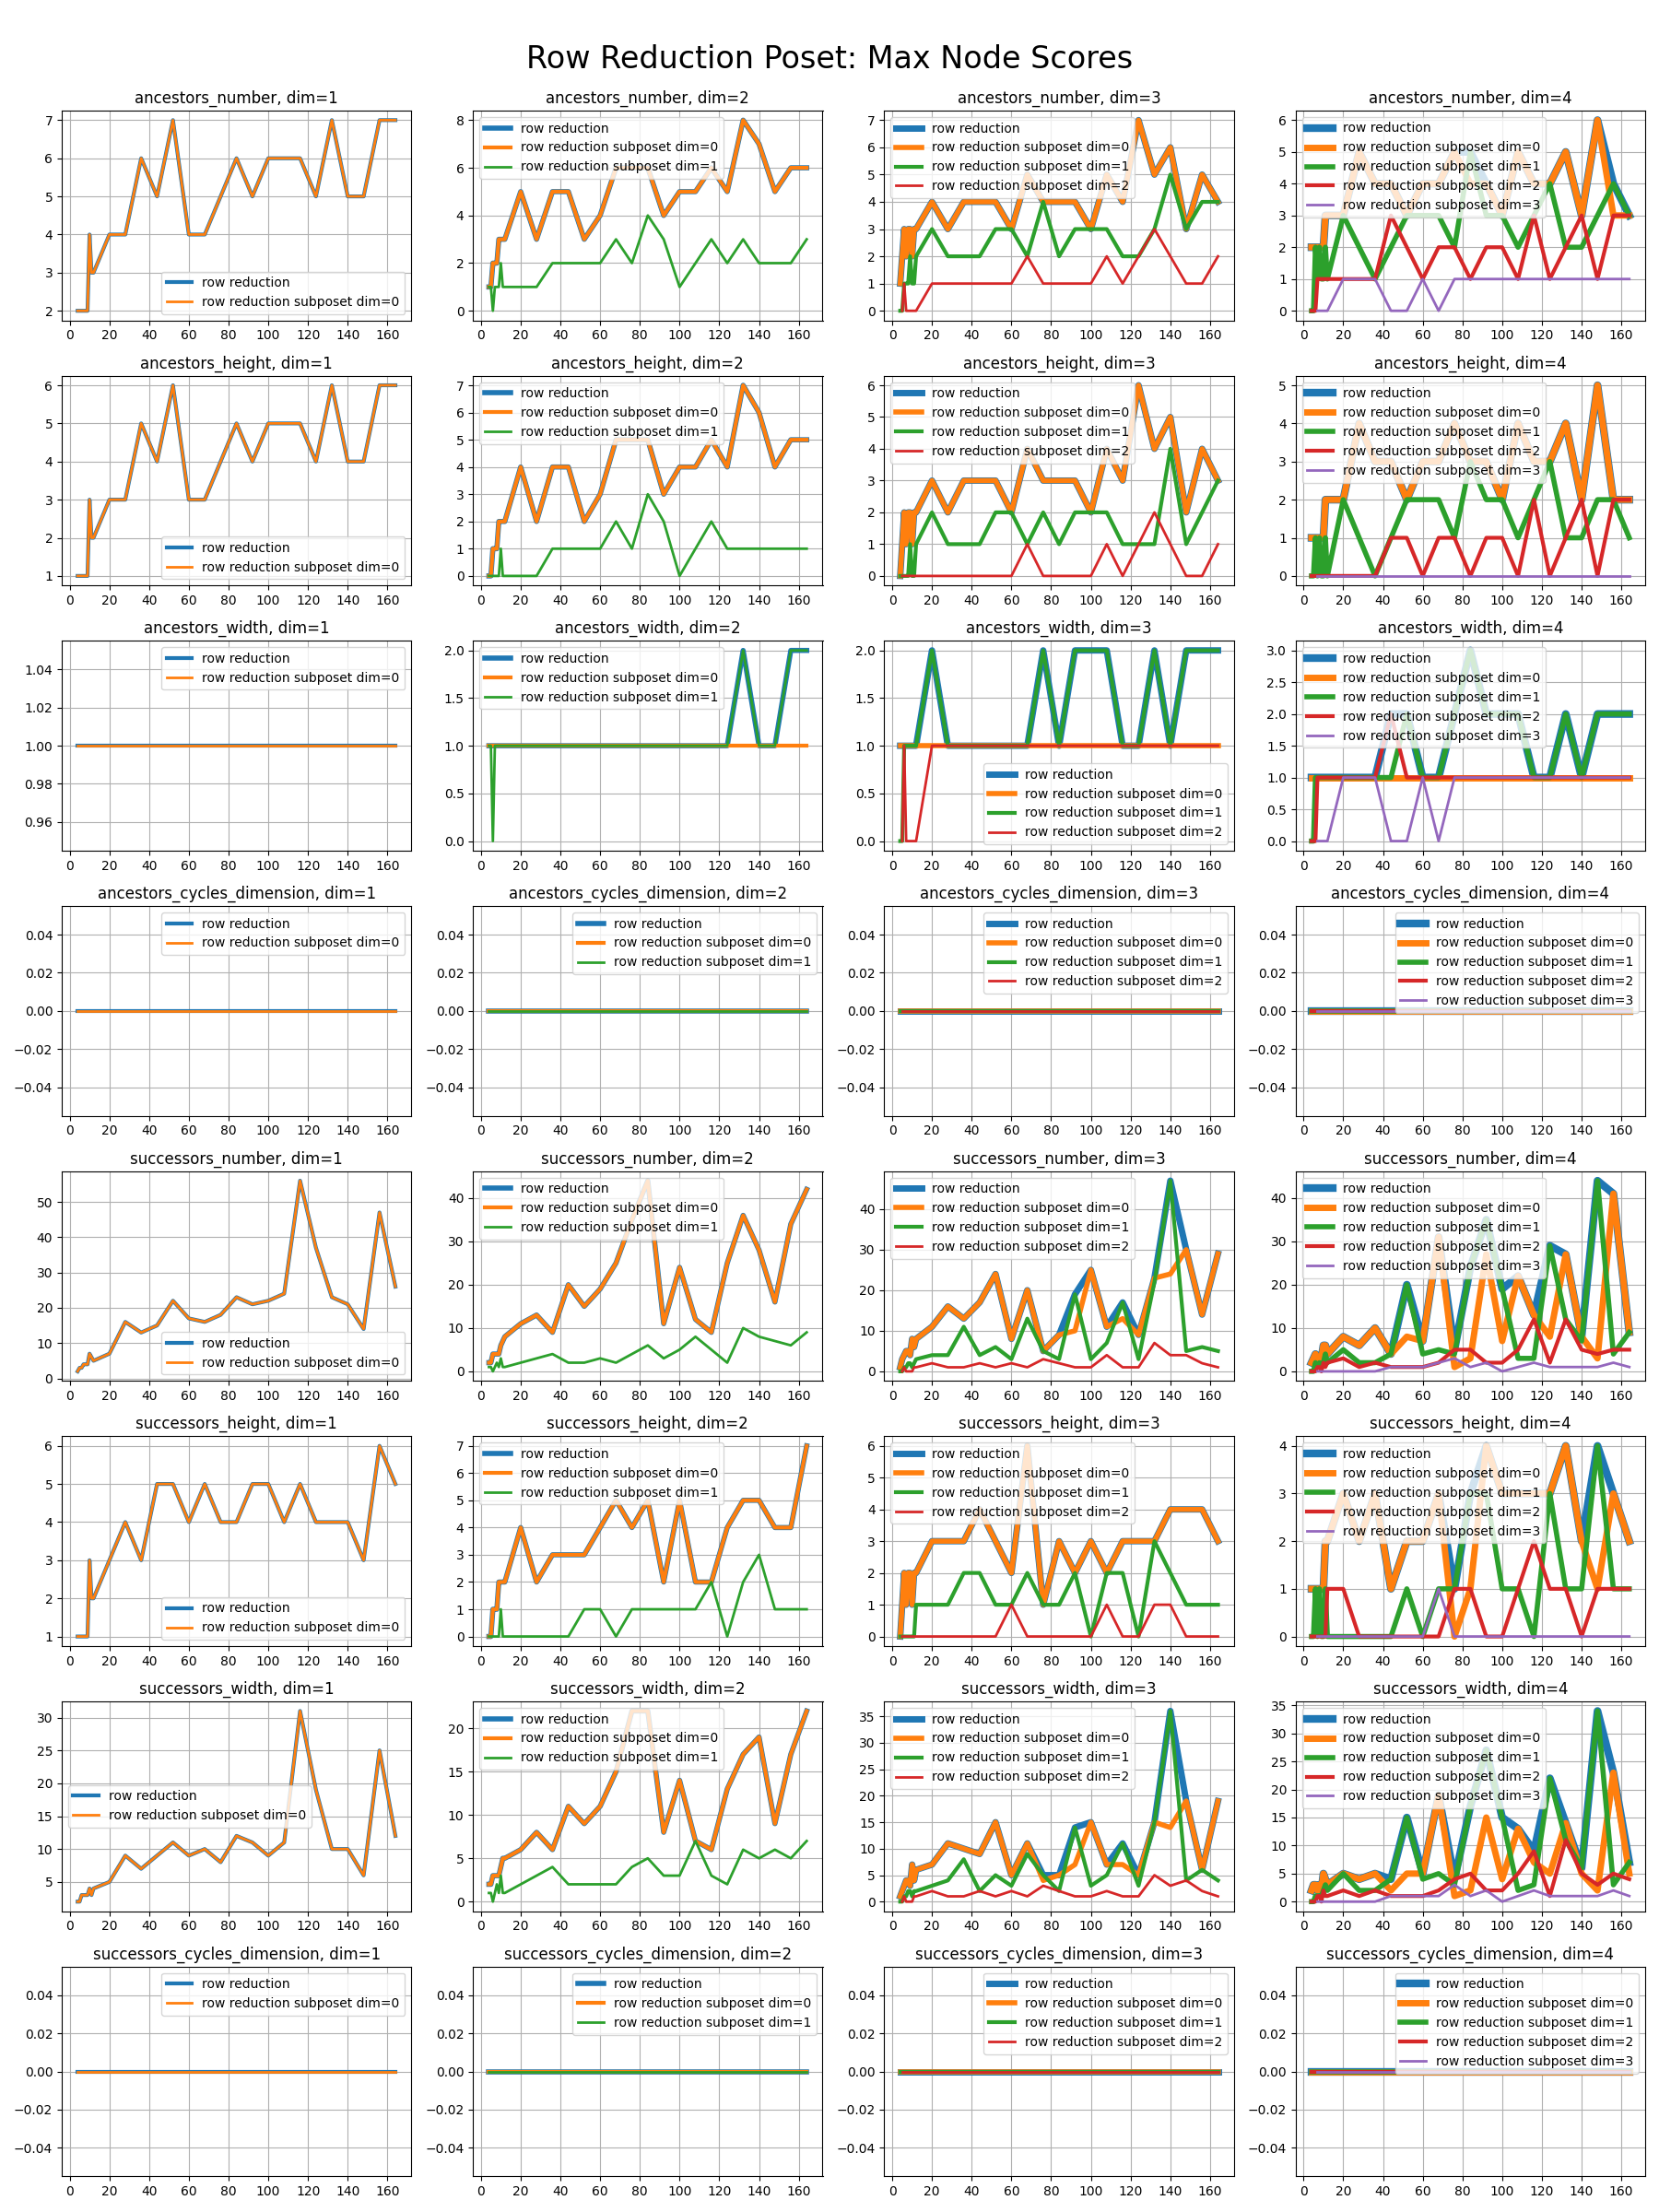
\includegraphics[width=\textwidth]{pics/scores - max node scores - row reduction.png}}
  \caption{Row Reduction Poset: Max node scores}
  \label{fig:scores_node_max_rrp}
\end{figure}

\section{Conclusion}
\par Row and Column reduction posets for d-dimensional case can have cycles, but their subposets with pairs dimension d-1 (where the dimension of a pair corresponds to the lower dimension of a simplex) are always trees.



\end{document}